\documentclass{article}
\usepackage{amsmath, amssymb, mathtools, bm}
\usepackage{graphicx, graphics}
\usepackage{array}
\DeclareMathOperator*{\argmin}{arg\,min}

\title{PyKE: Open source Python data analysis for NASA's Kepler, K2, and TESS missions}
\author{PyKE Contributors}
\date{\today}

\begin{document}
\maketitle

\begin{abstract}

\end{abstract}

\section{Introduction}

\section{Lightcurve Basics}
    \subsection{The \texttt{LightCurve} class}
        A \texttt{LightCurve} object can be instantiated by passing a \texttt{time}
        array, a \texttt{flux} array, and optionally a \texttt{flux\_err} array which
        accounts for uncertainties in the \texttt{flux} measurements, i.e.,
        \begin{verbatim}
        from pyke.lightcurve import LightCurve
        lc = LightCurve(time, flux)
        \end{verbatim}

        The \texttt{LightCurve} object provides methods described in
        Table~(\ref{tab:methods}).

        \begin{table}[!htb]
            \centering
            \caption{A subset of methods provided by the \texttt{LightCurve} class}
            \begin{tabular}{cp{7cm}}
                \hline
                \textbf{Method signature} & \textbf{Short description} \\
                \hline
                \texttt{stitch} & appends the attributes \texttt{flux},
                \texttt{time}, and \texttt{flux\_err} of other given
                \texttt{LighCurve} objects.\\
                \texttt{flatten} & applies a Savitzky-Golay filter to capture
                low frequency flux variations which can be then removed in order
                to aid transit detection algorithms.\\
                \texttt{fold} & folds a lightcurve at a given period and phase.\\
                \texttt{bin} &  bins a lightcurve using a block mean or median.\\
                \texttt{cdpp} &  computes the Combined Differential Photometric
                Precision (CDPP) metric, which is a proxy for the amount of
                scatter in the lightcurve signal. \\
                \texttt{plot} & displays a lightcurve.
            \end{tabular}
            \label{tab:methods}
        \end{table}

       The \texttt{KeplerLightCurve} class extends \texttt{LightCurve} by
       adding attributes to store metadata information such as channel number,
       quality flags, campaign or quarter number, kepler id, etc.

       Additionally, \texttt{KeplerLightCurve} can be corrected for motion-dependent
       correlated noise using the \texttt{correct} method which will be discussed in
       Section~\ref{subsection:motion}.

   \subsection{The \texttt{KeplerLightCurveFile} class}
        The \texttt{KeplerLightCurveFile} class defines a structure to deal
        with lightcurve files from both NASA's Kepler and K2 missions.

        To instantiate a \texttt{KeplerLightCurveFile} object, it is necessary
        to pass a \texttt{path} which represents the address (url or local path)
        of a lightcurve file in the fits (or compressed) format, and a
        \texttt{quality\_bitmask} string which specifies quality
        flags of cadences that should be ignored.

        One crucial method of the \texttt{KeplerLightCurveFile} class is
        \texttt{get\_lightcurve} which returns a \texttt{KeplerLightCurve} object
        with the metadata provided by the corresponding \texttt{KeplerLightCurveFile}.

        Therefore, one can, for example, perform the following series of operations
        in order to fold a lightcurve from the MAST archive
\begin{verbatim}
>>> lc_file = KeplerLightCurveFile("https://archive.stsci.edu/missions/kepler/"
... "lightcurves/0119/011904151/kplr011904151-2009350155506_llc.fits")
>>> klc = lc_file.get_lightcurve("PDCSAP_FLUX").fold(period=10.8234)
>>> klc.plot()
\end{verbatim}
        \begin{figure}[!htb]
            \centering
            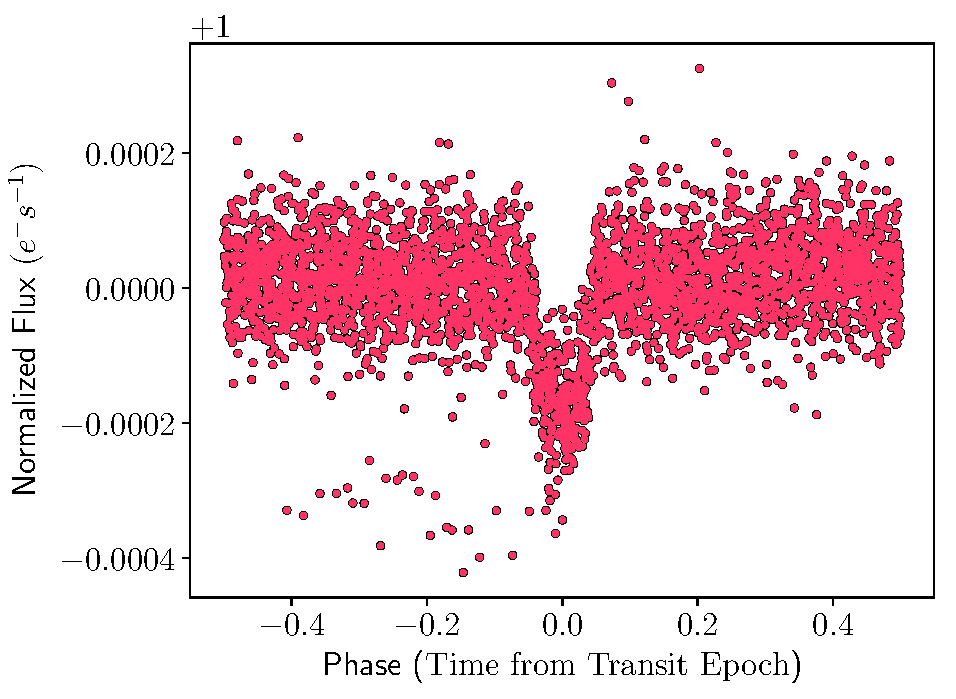
\includegraphics[scale=.5]{figs/fold-lc.pdf}
            \caption{Folded lightcurve of target \texttt{KIC011904151} quarter 3, showing the
            transit signal of Kepler-10b.}
            \label{fig:fold-method}
        \end{figure}

\section{Target Pixel File Basics}
    \subsection{The \texttt{KeplerTargetPixelFile} class}
        A \texttt{KeplerTargetPixelFile} object can be instantiated
        by passing a \texttt{path} (URL or local) of a target pixel file.
        Optionally, the user can elect to throw away frames that contain
        a specific flag by using the \texttt{quality\_bitmask} argument.

        \texttt{KeplerTargetPixelFile} offers a number of methods
        that range from getting raw aperture photometry lightcurves to
        data visualization.

        For instance, the method \texttt{plot} can be used to visualize a
        given frame, which are depicted in Fig.~\ref{fig:plot-method}
\begin{verbatim}
import numpy as np
from pyke import KeplerTargetPixelFile
tpf = KeplerTargetPixelFile('kplr008462852-2011073133259_lpd-targ.fits.gz')
tpf.plot()
tpf.plot(aperture_mask=tpf.flux[0] > np.nanmean(tpf.flux[0]))
\end{verbatim}

        \begin{figure}[!htb]
            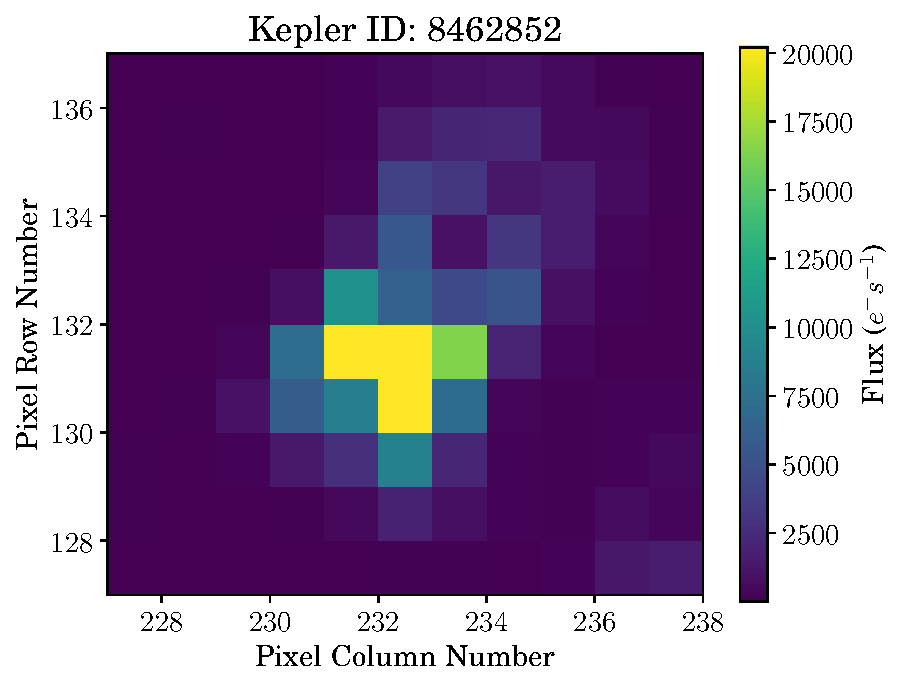
\includegraphics[scale=.4]{figs/tpf-plot.pdf}
            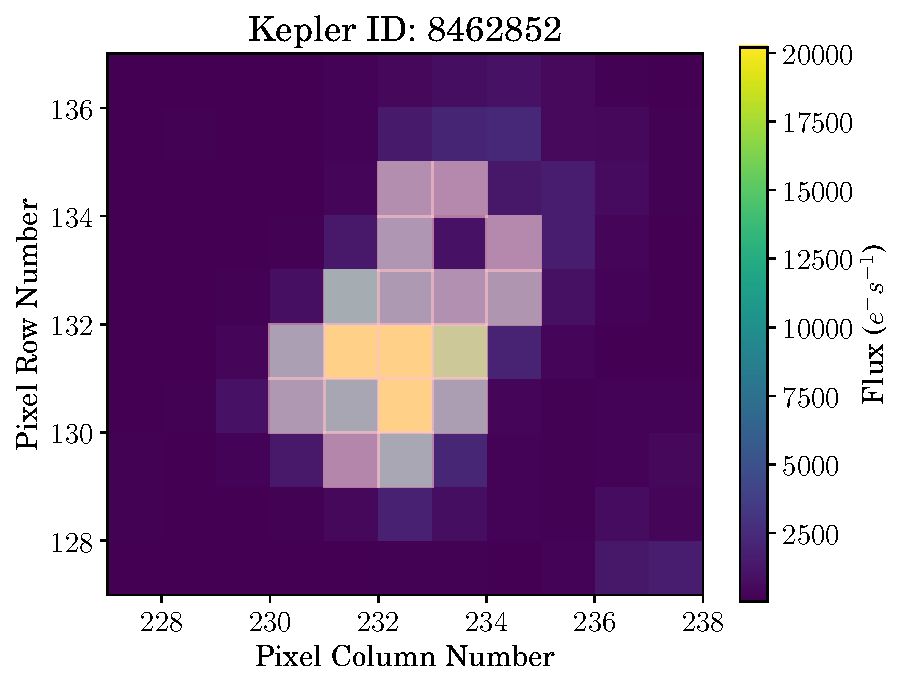
\includegraphics[scale=.4]{figs/tpf-plot-aperture.pdf}
            \caption{}
            \label{fig:plot-method}
        \end{figure}


\section{Tools}

\subsection{Cotrending basis vectors}

Cotrending basis vectors (CBVs) can remove global correlated
systematics present in a given channel \cite{2012PASP..124.1000S}.

Given a set of $n$ CBVs, one is interested in finding a set of $n$
coefficients $\bm{\theta}=(\theta_1, \theta_2, ..., \theta_n)$ which minimizes
some cost function between the SAP flux and the set of CBVs.

The following cost function is often used
\begin{align}
    \bm{\theta}^{*} = \argmin_{\bm{\theta} \in \Theta} \sum_{t}|f_{SAP}(t)
    - \sum_{j=1}^{n}\theta_j v_{j}(t)|^p, p>0, p \in \mathbb{R},
\end{align}
in which $f_{SAP}$ is the SAP flux and $v_j$ is the $j$-th CBV.

Then, the CBV-corrected flux can be computed as
\begin{equation}
    f_{CBV} = f_{SAP} - \sum_{j=1}^{n}\theta^{*}_j v_{j}(t).
\end{equation}

An example of SAP flux correction for target \texttt{KOI 8462852}
can be written as follows
\begin{verbatim}
from pyke.lightcurve import KeplerCBVCorrector
cbv = KeplerCBVCorrector("https://archive.stsci.edu/missions/kepler/lightcurves/"
                         "0084/008462852/kplr008462852-2011073133259_llc.fits")
cbv_lc = cbv.correct(cbvs=[1,2])
\end{verbatim}

Fig~\ref{fig:cbv-correction} illustrates the CBV correction.
\begin{figure}[!htb]
    \centering
    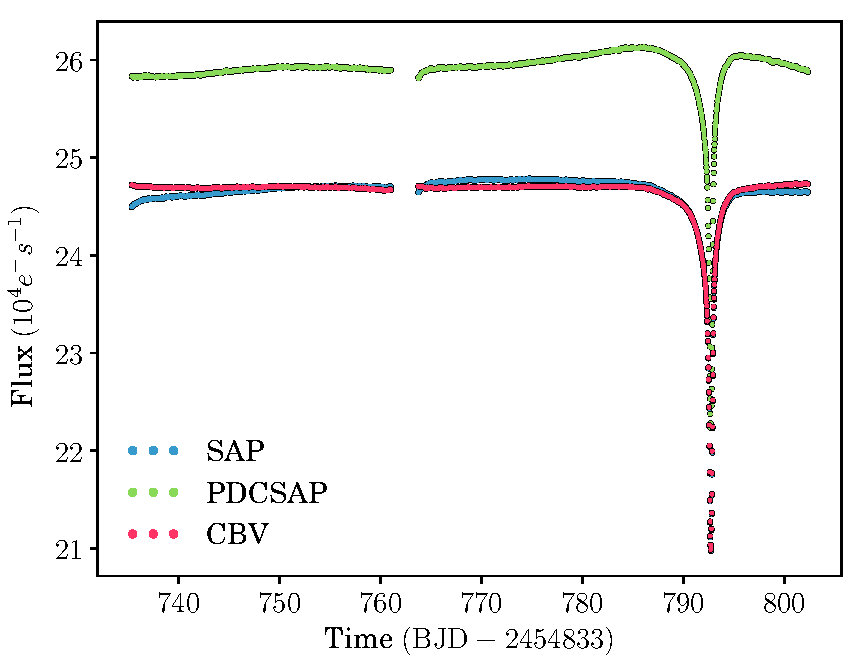
\includegraphics[scale=.5]{figs/cbv.pdf}
    \caption{CBV correction applied on \texttt{KOI 8462852}}
    \label{fig:cbv-correction}
\end{figure}

In this setting, the user is left to choose the cost function and the number
of CBVs. Experimentation showed that $p=1$ yields robust (non-overfitted)
results; $p=1$ defines the outlier-resilient $\ell_1$-norm
\cite{2014sdmm.book.....I}.

Improperly tuning the number of CBVs can cause over-/under-fitting. One
way to identify a reasonable number of CBVs is to perform a grid search
as shown in Fig~(\ref{fig:cbv-grid-search}).

\begin{figure}[!htb]
    \centering
    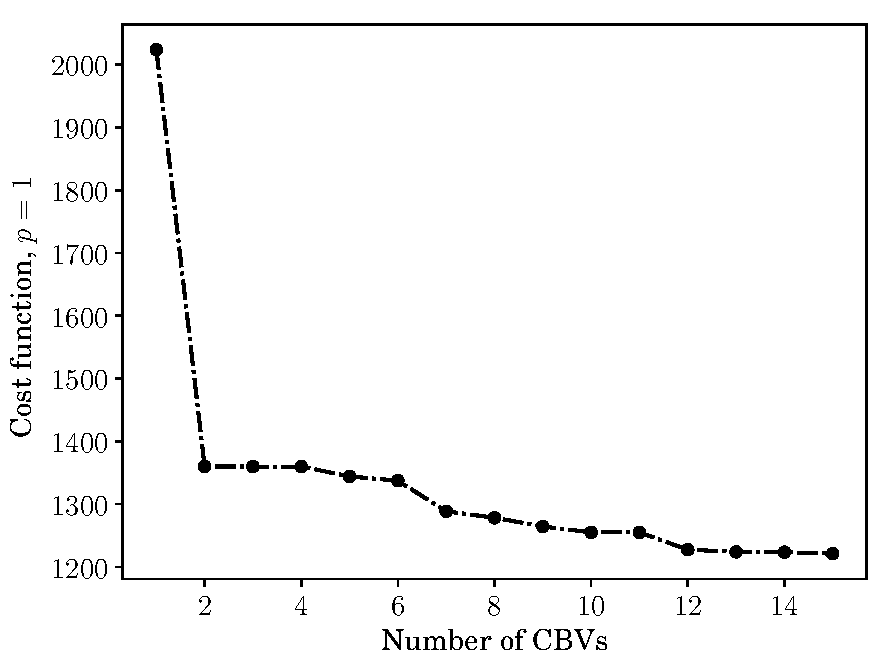
\includegraphics[scale=.5]{figs/cbv-grid-search.pdf}
    \caption{Grid search on the number of CBVs}
    \label{fig:cbv-grid-search}
\end{figure}

We can similarly apply cotrending basis vector correction to
 lightcurves.

Fig.~\ref{fig:cbv-correction-k2} shows the detrended lightcurve after estimating
the first nine coefficients for CBV correciton on $\mathcal{K}\mathit{2}$ target
 \texttt{EPIC 201543306}. The selection of the number of CBVs is set by inspecting the
grid search curve can be set through model comparison heuristics like AIC, BIC,
or cross-validation \cite{2014sdmm.book.....I}.

% MGS note: Wait--- won't the cost function decrease monotonically for CBVs?
% Do you use AIC or BIC or cross-validation?

\begin{figure}[!htb]
    \centering
    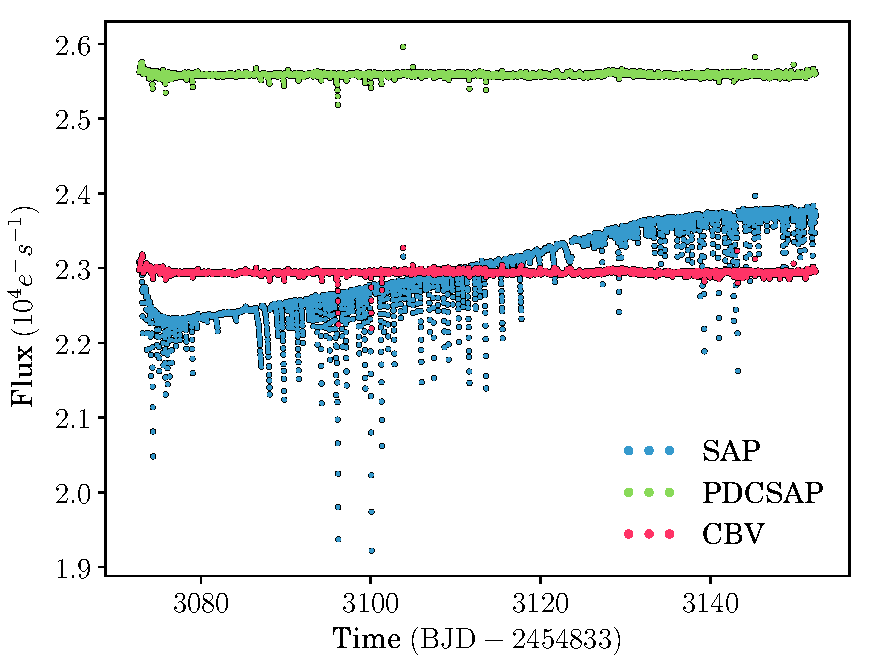
\includegraphics[scale=.5]{figs/cbv-k2.pdf}
    \caption{CBV correction applied on \texttt{EPIC 201543306}.}
    \label{fig:cbv-correction-k2}
\end{figure}

\subsection{Point spread function photometry}

PyKE contains routines to perform PSF photometry in TPFs
which are implemented in the \texttt{psf} module.

Briefly, the PSF photometry problem that PyKE solves can be formulated as
follows. Given an image $\bm{y}$, with $n$ pixels and $m$ stars, and a PSF model
$\lambda(\bm{\theta}) = \sum_{j=1}^{m} \lambda({\theta}_j)$,
find the best parameter vector
$\bm{\theta}^{*} = (\theta_1^{*}, \theta_2^{*}, ..., \theta_m^{*})$
that minimizes some cost (or loss) function $R(\lambda(\bm{\theta}), \bm{y})$
of assigning $\bm{\theta} = \bm{\theta}^{*}$.

The example below illustrates PSF photometry on the target \texttt{EPIC 246199087}
(Trappist-1):

\begin{verbatim}
from pyke import KeplerTargetPixelFile
from pyke.psf import PRFPhotometry, SceneModel
from oktopus import UniformPrior

tpf = KeplerTargetPixelFile("ktwo246199087-c12_lpd-targ.fits.gz")
prf = tpf.get_prf_model()
prior = UniformPrior(lb=[4e3, 990, 25, 1], ub=[2e4, 996, 30, 2e3])
scene = SceneModel(prf=[prfs])

phot = PRFPhotometry(scene_model=scene, prior=prior)
results = phot.fit(tpf.flux + tpf.flux_bkg)
\end{verbatim}

The photometric results are stored in a $c \times 4$ matrix, where $c$ is the
number of frames (cadences).

From a probabilistic point of view, one is often interested in minimizing the
expected cost with respect to some probability distribution assigned to the data
$\bm{y}$ and to the parameter vector $\bm{\theta}$, from which the cost function
$R$ naturally arises. The default assumption on the data is that it follows
a Poisson probability distribution; whereas the probability distribution on the
parameter vector has to be assigned by the user using the $\texttt{prior}$
argument.

Another important aspect is the PSF model...

\subsection{Motion-dependent Correlated Noise}

Spacecraft-induced correlated noise remains one of the greatest hurdles to analyzing K2 lightcurves.  Many algorithms have been developed to mitigate motion-dependent artifacts \cite{vanderburg14}.  Local and global Gaussian Process covariance kernels...

\label{subsection:motion}

\section{Acknowledgments}
PyKE is build on top of numerous packages that constitute the Python scientific
stack, more precisely, \texttt{numpy}, \texttt{scipy}, \texttt{matplotlib}, and
\texttt{astropy}.

\clearpage

%% MGS 2/2018: Uncomment below to enable references.
%\bibliographystyle{aasjournal}
%\bibliography{ms}

\end{document}
